%%%%%%%%%%%%%%%%%%%%%%%%%%%%%%%%%%%%%%%%%
% Jacobs Landscape Poster
% LaTeX Template
% Version 1.0 (29/03/13)
%
% Created by:
% Computational Physics and Biophysics Group, Jacobs University
% https://teamwork.jacobs-university.de:8443/confluence/display/CoPandBiG/LaTeX+Poster
%
% Further modified by:
% Nathaniel Johnston (nathaniel@njohnston.ca)
%
% This template has been downloaded from:
% http://www.LaTeXTemplates.com
%
% License:
% CC BY-NC-SA 3.0 (http://creativecommons.org/licenses/by-nc-sa/3.0/)
%
%%%%%%%%%%%%%%%%%%%%%%%%%%%%%%%%%%%%%%%%%

%----------------------------------------------------------------------------------------
%   PACKAGES AND OTHER DOCUMENT CONFIGURATIONS
%----------------------------------------------------------------------------------------

\documentclass[final]{beamer}

\usepackage{tikz}
\usepackage{newtxtext,newtxmath} % nice math font; optional


\usepackage[scale=1.24]{beamerposter} % Use the beamerposter package for laying out the poster
\usepackage{amsmath}
\usepackage{braket}
\usetheme{confposter} % Use the confposter theme supplied with this template

\usetikzlibrary{arrows.meta,calc,angles,quotes}

\setbeamercolor{block title}{fg=ngreen,bg=white} % Colors of the block titles
\setbeamercolor{block body}{fg=black,bg=white} % Colors of the body of blocks
\setbeamercolor{block alerted title}{fg=white,bg=dblue!70} % Colors of the highlighted block titles
\setbeamercolor{block alerted body}{fg=black,bg=dblue!10} % Colors of the body of highlighted blocks
% Many more colors are available for use in beamerthemeconfposter.sty

%-----------------------------------------------------------
% Define the column widths and overall poster size
% To set effective sepwid, onecolwid and twocolwid values, first choose how many columns you want and how much separation you want between columns
% In this template, the separation width chosen is 0.024 of the paper width and a 4-column layout
% onecolwid should therefore be (1-(# of columns+1)*sepwid)/# of columns e.g. (1-(4+1)*0.024)/4 = 0.22
% Set twocolwid to be (2*onecolwid)+sepwid = 0.464
% Set threecolwid to be (3*onecolwid)+2*sepwid = 0.708

\newlength{\sepwid}
\newlength{\onecolwid}
\newlength{\twocolwid}
\newlength{\threecolwid}
\setlength{\paperwidth}{48in} % A0 width: 46.8in
\setlength{\paperheight}{36in} % A0 height: 33.1in
\setlength{\sepwid}{0.024\paperwidth} % Separation width (white space) between columns
\setlength{\onecolwid}{0.22\paperwidth} % Width of one column
\setlength{\twocolwid}{0.464\paperwidth} % Width of two columns
\setlength{\threecolwid}{0.708\paperwidth} % Width of three columns
\setlength{\topmargin}{-0.5in} % Reduce the top margin size
%-----------------------------------------------------------


\usepackage{graphicx}  % Required for including images

\usepackage{booktabs} % Top and bottom rules for tables

%----------------------------------------------------------------------------------------
%   TITLE SECTION
%----------------------------------------------------------------------------------------

\title{Configurational Coupled Cluster for Planar Rotors} % Poster title

\author{Illia Voropai, Azharuddin Mohammed, Marcel Nooijen} % Author(s)

\institute{Department of Chemistry, University of Waterloo} % Institution(s)

%----------------------------------------------------------------------------------------

\begin{document}

\addtobeamertemplate{block end}{}{\vspace*{2ex}} % White space under blocks
\addtobeamertemplate{block alerted end}{}{\vspace*{2ex}} % White space under highlighted (alert) blocks

\setlength{\belowcaptionskip}{2ex} % White space under figures
\setlength\belowdisplayshortskip{2ex} % White space under equations

\begin{frame}[t] % The whole poster is enclosed in one beamer frame

\begin{columns}[t] % The whole poster consists of three major columns, the second of which is split into two columns twice - the [t] option aligns each column's content to the top

\begin{column}{\sepwid}\end{column} % Empty spacer column

\begin{column}{\onecolwid} % The first column

%----------------------------------------------------------------------------------------
%   OBJECTIVES
%----------------------------------------------------------------------------------------


%----------------------------------------------------------------------------------------
%   INTRODUCTION
%----------------------------------------------------------------------------------------
\begin{block}{Premise}

We would like to use the time idependent Schrodinger Equation to extract eigenvalues and eigenvectors.


\begin{equation}
\hat{H} = B \hat{K} + g\hat{V}
\end{equation}

Where hamiltonian describes a coplanar rotor system.

\begin{tikzpicture}[line cap=round,line join=round]
  % ----- styles & colors -----
    \definecolor{diskfill}{RGB}{160,175,200}  % blue-gray
  \tikzset{
    disk/.style={draw=black,fill=diskfill,thick},
    axis/.style={draw=black,-{Stealth[scale=1]}},
    dashline/.style={draw=black,dash pattern=on 7pt off 7pt},
    arr/.style={draw=black,-{Stealth[scale=1]}}
  }

  % ----- geometry -----
  \def\R{2}              % disk radius
  \coordinate (C1) at (0,0);
  \coordinate (C2) at (6,0);
  \coordinate (C3) at (12,0);
  \coordinate (C4) at (18,0);



  % ----- the four disks -----
  \foreach \C in {C1,C2,C3,C4}{
    \draw[disk] (\C) circle (\R);
  }

  % dashed baseline through centers
  \draw[line width=2.5pt, dashline] (-1,0) -- (19.5,0);

  % small arrows in disks (you can tweak angles/lengths)
  % Disk 1: short arrow slightly above baseline
  \draw[line width=2pt, arr] ($(C1)$) -- ($(C1)+(1.959,0.4)$);

  % Disk 2: arrow pointing up-right
  \draw[line width=2pt, arr] ($(C2)$) -- ($(C2)+(1.5,1.322)$);

  % Disk 3: arrow pointing up-right
  \draw[line width=2pt, arr] ($(C3)$) -- ($(C3)+(-1,1.732)$);

  % Disk 4: arrow down-right
  \draw[line width=2pt, arr] ($(C4)$) -- ($(C4)+(-1,-1.732)$);

  % ----- axes on the right -----
  \coordinate (O) at (21,0);
  \draw[line width=2.5pt, axis] (O) -- ++(2,0) node[below right=-1pt] {\(x\)};
  \draw[line width=2.5pt, axis] (O) -- ++(0,2) node[above left=-1pt] {\(y\)};

\end{tikzpicture}

We solve Shrodinger equation by diagnilizing hamiltonian:

\begin{align}
    \hat{H}\ket{\psi} &= E\ket{\psi}
\end{align}

However thise hamiltonians becove extreamly large really fast which makes exact diagnilization computationally heavy.

\textit{(Even though we are curently working with systems of rotors the method is equaly aplicable to magnetic systems.)}

\begin{alertblock}{Problem Statement}
Generalize Coupled Cluster methods (CC) to rotor systems, to explore larger systems. Compare with other approaches and also consider Thermal Properties.
\end{alertblock}

\end{block}

\begin{block}{Improving Exact Diagonilization}
In order to to explore larger systems with Exact Diagnilization and Configurational Coupled Cluster (CCC) we use Natural Orbitals:
\begin{itemize}
  \item Truncate the basis using Natural Orbital (NO) density matrix for small system(2-3 sites), and use selected eivencectors.
  \item Use sparse matrix techniquesto COnstruct Hamiltonian and use direct diagnilization.
  \item Systems up to about 9 sites with 3-5 NO's can be studied.
\end{itemize}

\begin{figure}
    \centering
    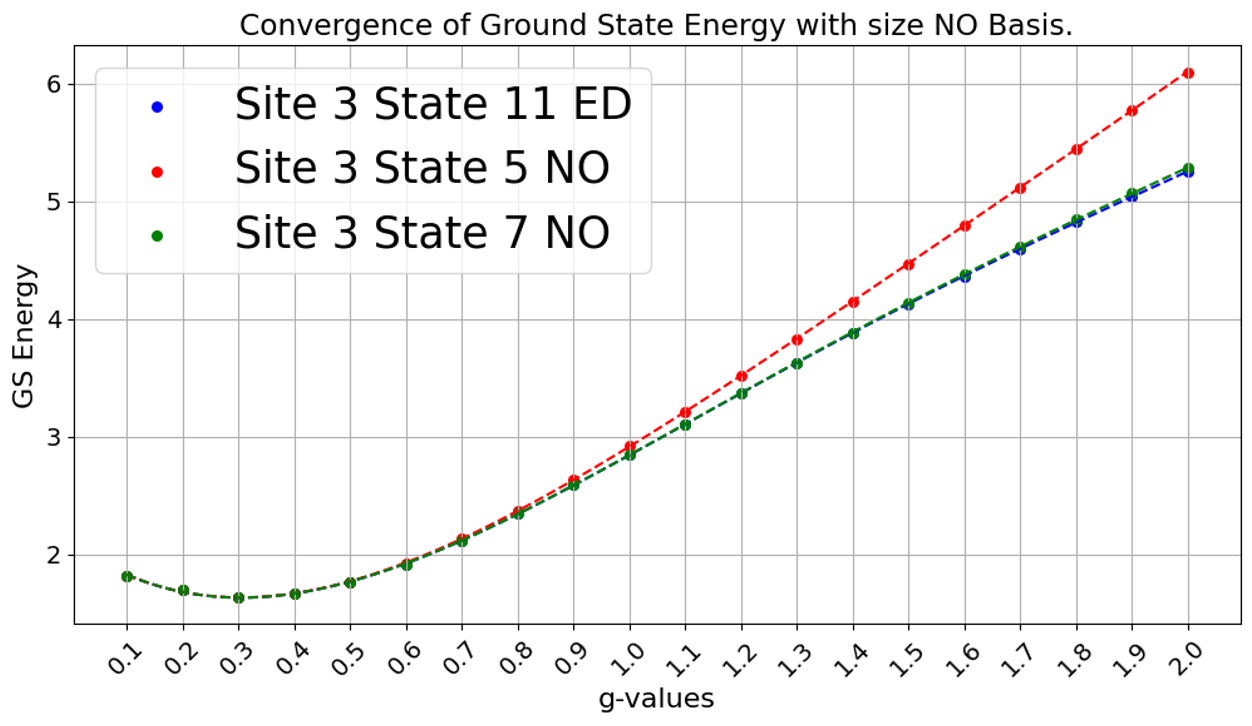
\includegraphics[width=.9\linewidth]{ED_vs_NO.png}
    \caption{Qualitative demonstration works through the NO truncation method but acuracy decreases with the increase of the coupling strengs.}
    \label{fig:ED_vs_NO}
\end{figure}

\end{block}
%------------------------------------------------

%----------------------------------------------------------------------------------------


\end{column} % End of the first column

\begin{column}{\sepwid}\end{column} % Empty spacer column

\begin{column}{\twocolwid} % Begin a column which is two columns wide (column 2)

\begin{columns}[t,totalwidth=\twocolwid] % Split up the two columns wide column

\begin{column}{\onecolwid}\vspace{-.6in} % The first column within column 2 (column 2.1)

%----------------------------------------------------------------------------------------
%   MATERIALS
%----------------------------------------------------------------------------------------

\begin{block}{Periodic vs. Non-Periodic System Setup}

CCC calcualations can be sued for both periodic and finite systems. One could go beyond nearest neighbor interactions.

The example of the periodic system that we would consider:



\begin{figure}

\text{Periodic}\par\vspace{0.5em}

\definecolor{diskfill}{RGB}{160,175,200}  % blue-gray nodes
\definecolor{arrowblue}{RGB}{35,85,170}   % arrow color
\def\lw{1.2pt}                            % line thickness
\def\R{0.9}                              % node radius

\tikzset{
  hop/.style={draw=arrowblue, line width=\lw,
              {Stealth[scale=1]}-{Stealth[scale=1]}},
  hopdotted/.style={hop, dotted},                % dotted hop (last one)
  basearc/.style={draw=arrowblue!70, line width=\lw, dashed, {Stealth[scale=1]}-{Stealth[scale=1]}},
  nodept/.style={draw=arrowblue!70!black, fill=diskfill,
                 line width=\lw, circle, minimum size=2*\R, inner sep=10pt},
  ghostpt/.style={draw=arrowblue, line width=\lw, dashed, circle}
}


  % ---- figure ----
  \begin{tikzpicture}[line cap=round, line join=round, x=4cm, y=2.0cm]
  % positions 0..6 along x-axis at y=0
  \foreach \i in {0,...,5}{
    \node[nodept] (P\i) at (\i,0) {};
  }
  % ghost node at x=6 (dotted outline)
  \draw[ghostpt] (6,0) circle (13pt);

  % semicircle hops (solid) from i -> i+1 for i=0..4
  % use arc centered at (i+0.5,0): start at angle 180, end at 0, radius=0.5
  \foreach \i in {0,...,4}{
    \draw[hop] (\i,0.25) arc[start angle=180, end angle=0, radius=0.5];
  }
  % last hop (dotted) from 5 -> 6
  \draw[hopdotted] (5,0.25) arc[start angle=180, end angle=0, radius=0.5];

  % long dashed “return” arc from x=0 to x=6 (slightly below)
  % gentle sag using control points; tweak if you want more/less curvature
  \draw[basearc] (0,-0.25) .. controls (0.5,-1) and (4.5,-1) .. (5,-0.25);

  % labels above each solid node
\node[below=-15pt, align=center, font=\fontsize{15}{15}\selectfont]
     at (0.5,0.5) {$x=1$\\$y=2$};

\node[below=-15pt, align=center, font=\fontsize{15}{15}\selectfont]
     at (1.5,0.5) {$x=2$\\$y=3$};

\node[below=-15pt, align=center, font=\fontsize{15}{15}\selectfont]
     at (2.5,0.5) {$x=3$\\$y=4$};

\node[below=-15pt, align=center, font=\fontsize{15}{15}\selectfont]
     at (3.5,0.5) {$x=4$\\$y=5$};

\node[below=-15pt, align=center, font=\fontsize{15}{15}\selectfont]
     at (4.5,0.5) {$x=5$\\$y=6$};

\node[below=-15pt, align=center, font=\fontsize{15}{15}\selectfont]
     at (5.5,0.5) {$x=6$\\$y=7$};

  % label under the long dashed arc
  \node[above=-22pt, align=center, font=\fontsize{15}{15}\selectfont] at (2.5,-0.6) {$x=6$\\$y=0$};
\end{tikzpicture}


\text{Non-Periodic}\par\vspace{0.5em}


\definecolor{diskfill}{RGB}{160,175,200}  % blue-gray nodes
\definecolor{arrowblue}{RGB}{35,85,170}   % arrow color
\def\lw{1.2pt}                            % line thickness
\def\R{0.9}                              % node radius

\tikzset{
  hop/.style={draw=arrowblue, line width=\lw,
              {Stealth[scale=1]}-{Stealth[scale=1]}},
  hopdotted/.style={hop, dotted},                % dotted hop (last one)
  basearc/.style={draw=arrowblue!70, line width=\lw, dashed, {Stealth[scale=1]}-{Stealth[scale=1]}},
  nodept/.style={draw=arrowblue!70!black, fill=diskfill,
                 line width=\lw, circle, minimum size=2*\R, inner sep=10pt},
  ghostpt/.style={draw=arrowblue, line width=\lw, dashed, circle}
}

% ---- figure ----
\begin{tikzpicture}[line cap=round, line join=round, x=4cm, y=2.0cm]
  % positions 0..6 along x-axis at y=0
  \foreach \i in {0,...,5}{
    \node[nodept] (P\i) at (\i,0) {};
  }

  % semicircle hops (solid) from i -> i+1 for i=0..4
  % use arc centered at (i+0.5,0): start at angle 180, end at 0, radius=0.5
  \foreach \i in {0,...,4}{
    \draw[hop] (\i,0.25) arc[start angle=180, end angle=0, radius=0.5];
  }

  % labels above each solid node
\node[below=-15pt, align=center, font=\fontsize{15}{15}\selectfont]
     at (0.5,0.5) {$x=1$\\$y=2$};

\node[below=-15pt, align=center, font=\fontsize{15}{15}\selectfont]
     at (1.5,0.5) {$x=2$\\$y=3$};

\node[below=-15pt, align=center, font=\fontsize{15}{15}\selectfont]
     at (2.5,0.5) {$x=3$\\$y=4$};

\node[below=-15pt, align=center, font=\fontsize{15}{15}\selectfont]
     at (3.5,0.5) {$x=4$\\$y=5$};

\node[below=-15pt, align=center, font=\fontsize{15}{15}\selectfont]
     at (4.5,0.5) {$x=5$\\$y=6$};

\end{tikzpicture}
\caption{Circles representing rotor sites, x and y respresenting site interactions between sites 1 and 2; 2 and 3: etc.  The doted lines and sites are two ways how we can consider our periodic systems}
\label{fig:non_periodic_system_drawing}
\end{figure}


\end{block}

\begin{block}{Configurational Coupled Cluster}

    - CI CCC comparison emfesising the separated exictation operators and ability of CCC to axes higher excitations.



\end{block}

%----------------------------------------------------------------------------------------

\end{column} % End of column 2.1

\begin{column}{\onecolwid}\vspace{-.6in} % The second column within column 2 (column 2.2)

%----------------------------------------------------------------------------------------
%   METHODS
%----------------------------------------------------------------------------------------

\begin{block}{Large $g >= 100$ Limit}

One of the properties which we utilise to explore the large g limit ($g>=100$) is that as g aproaches infininty the system becomes a superposition of two states (alignments) 0 and $\pi$.

\begin{figure}
\begin{tikzpicture}[line cap=round,line join=round]
  % ----- styles & colors -----
    \definecolor{arrow}{RGB}{232, 19, 40}  % blue-gray
    \definecolor{diskfill}{RGB}{160,175,200}  % blue-gray
  \tikzset{
    disk/.style={draw=black,fill=diskfill,thick},
    dashline_left/.style={draw=black, -{Stealth[scale=1]}, dash pattern=on 7pt off 7pt},
    dashline_right/.style={draw=black, {Stealth[scale=1]}-, dash pattern=on 7pt off 7pt},
    arr/.style={draw=arrow,-{Stealth[scale=1]}}
  }

  % ----- geometry -----
  \def\R{2}              % disk radius
  \coordinate (C1) at (0,-2);
  \coordinate (C2) at (6,-2);
  \coordinate (C3) at (12,-2);
  \coordinate (C4) at (18,-2);
  \coordinate (C5) at (0,-9);
  \coordinate (C6) at (6,-9);
  \coordinate (C7) at (12,-9);
  \coordinate (C8) at (18,-9);



  % ----- the four disks -----
  \foreach \C in {C1,C2,C3,C4,C5,C6,C7,C8}{
    \draw[disk] (\C) circle (\R);
  }

  % dashed baseline through centers
  \draw[line width=3pt, dashline_right] (-4,-2) -- (22,-2);

  \node[above=-22pt, align=center, font=\fontsize{25}{15}\selectfont] at (-1, 1) {alingnment = $0$};

  % dashed baseline through centers
  \draw[line width=3pt, dashline_left] (-4,-9) -- (22,-9);

  \node[above=-22pt, align=center, font=\fontsize{25}{15}\selectfont] at (-1,-5.5) {alingnment = $\pi$};


  \foreach \C in {C1,C2,C3,C4}{
    \draw[line width=3pt, arr] ($(\C)$) -- ($(\C)+(-2, 0)$);
  }

  \foreach \C in {C5,C6,C7,C8}{
    \draw[line width=3pt, arr] ($(\C)$) -- ($(\C)+(2, 0)$);
  }

\end{tikzpicture}
\caption{The shcematic for superposition of the two state alignments.}
\label{fig:superposition}
\end{figure}

With g large we can the wavefunctions assiciated with 0 and $\pi$ alignment are separate.
This property allows us to isolate for one of them in the following maner by taking a linear combination of the 0 and $\pi$ wavefunctions and constructing a Natural orbital basis based on them.

\begin{figure}
    \centering
    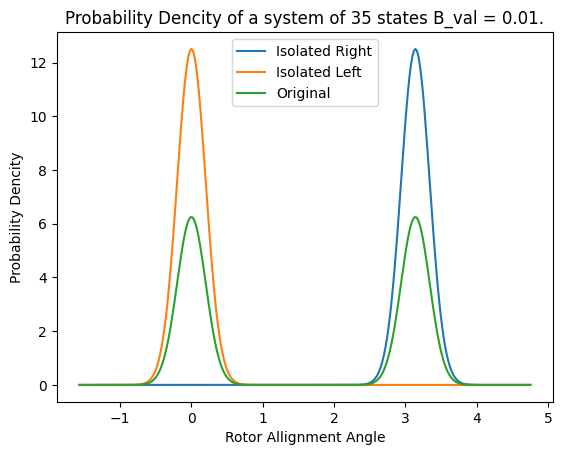
\includegraphics[width=.8\linewidth]{superposition_graph.png}
    \caption{The example of probability dencityes separated onto localised states instead of superposition.}
    \label{fig:superposition_graph}
\end{figure}

By solving the CCC equations for the system of Natural Orbital describing combined (isolated to the left or the right) state we can see a inverce prodoctional relationship between the value of B and the acuracy of CCC ground state energy.


\begin{figure}
    \centering
    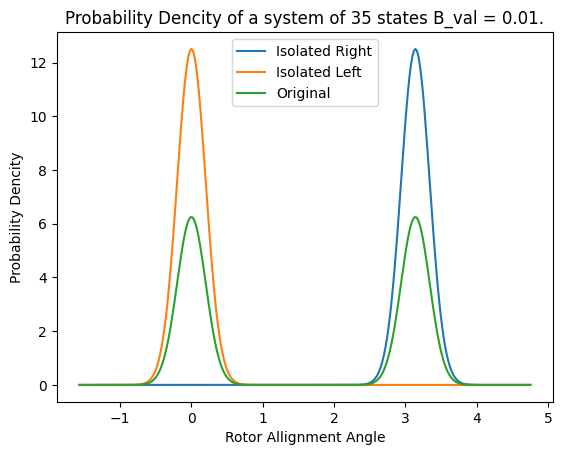
\includegraphics[width=.8\linewidth]{superposition_graph.png}
    \caption{As B aproaches 0 (g aproaches infinity) acuracy increases.}
    \label{fig:D_vs_CCC_Energy}
\end{figure}

\end{block}
%----------------------------------------------------------------------------------------

\end{column} % End of column 2.2

\end{columns} % End of the split of column 2 - any content after this will now take up 2 columns width


%----------------------------------------------------------------------------------------
%   IMPORTANT RESULTi
%----------------------------------------------------------------------------------------


%----------------------------------------------------------------------------------------

\begin{columns}[t,totalwidth=\twocolwid] % Split up the two columns wide column again

\begin{column}{\onecolwid} % The first column within column 2 (column 2.1)

%----------------------------------------------------------------------------------------
%   MATHEMATICAL SECTION
%----------------------------------------------------------------------------------------


%----------------------------------------------------------------------------------------

\end{column} % End of column 2.1

\begin{column}{\onecolwid} % The second column within column 2 (column 2.2)

%----------------------------------------------------------------------------------------
%   Future work
%----------------------------------------------------------------------------------------



%----------------------------------------------------------------------------------------

\end{column} % End of column 2.2

\end{columns} % End of the split of column 2

\end{column} % End of the second column

\begin{column}{\sepwid}\end{column} % Empty spacer column

\begin{column}{\onecolwid} % The third column

%--------------------------------------------------------------------------------

\begin{block}{Computational Efficency Results}

\end{block}

\begin{block}{Small $g < 100$ Limit}

\end{block}

\begin{block}{Future Work}

\end{block}


\begin{alertblock}{References}
    \small{\bibliographystyle{unsrt}
    \bibliography{sample}\vspace{0.75in}}
\end{alertblock}

%----------------------------------------------------------------------------------------
%   CONTACT INFORMATION
%----------------------------------------------------------------------------------------

\setbeamercolor{block alerted title}{fg=black,bg=norange} % Change the alert block title colors
\setbeamercolor{block alerted body}{fg=black,bg=white} % Change the alert block body colors

\begin{alertblock}{Contact Information}

\begin{itemize}
\item Email: \href{mailto:aas2999m@uwaterloo.ca}{aas2999m@uwaterloo.ca}
\end{itemize}

\end{alertblock}

\begin{center}
\begin{tabular}{ccc}
% \includegraphics[width=0.4\linewidth]{logo.png} & \hfill & \includegraphics[width=0.4\linewidth]{logo.png}
\end{tabular}
\end{center}

%----------------------------------------------------------------------------------------

\end{column} % End of the third column

\end{columns} % End of all the columns in the poster

\end{frame}  % End of the enclosing frame

\end{document}
